\documentclass[11pt,a4paper]{article}

% ---------- Packages ----------
\usepackage[utf8]{inputenc}
\usepackage[T1]{fontenc}
\usepackage{lmodern}
\usepackage{geometry}
\usepackage{float}
\usepackage{placeins}
\usepackage{caption}
\geometry{margin=1in}
\usepackage{setspace}
\onehalfspacing
\usepackage{graphicx}
\usepackage{hyperref}
\usepackage{csquotes}
\usepackage{enumerate}
\usepackage{xcolor}
\usepackage[style=authoryear,maxcitenames=2,backend=biber]{biblatex}

% ---------- Bibliography file ----------
\addbibresource{references.bib}

% ---------- Title ----------
\title{\textbf{The Rainy-Day Fund: Decentralized Parametric Insurance for Smallholder Farmers in Kenya}}
\author{
	Group A: Ellena, Sabina, Noah, Vincent\\[0.5em]
	\textit{University of Basel, Blockchain Challenge 25}
	}
	\date{\today}

	% ---------- Section formatting and ToC ----------
	\usepackage{titlesec}
	\usepackage{tocloft}
	\setcounter{secnumdepth}{3}
	\setcounter{tocdepth}{2}
	\titleformat{\section}
	{\Large\bfseries}{\thesection}{1em}{}
	\titlespacing*{\section}{0pt}{2.0ex plus .2ex minus .2ex}{1.0ex plus .2ex}
	\titleformat{\subsection}
	{\large\bfseries}{\thesubsection}{1em}{}
	\titlespacing*{\subsection}{0pt}{1.5ex plus .2ex minus .2ex}{0.8ex plus .2ex}
	\renewcommand{\cftsecfont}{\normalfont}
	\renewcommand{\cftsubsecfont}{\normalfont}
	\renewcommand{\cftsecpagefont}{\normalfont}
	\setlength{\cftbeforesecskip}{4pt}

	\begin{document}
	\maketitle

	\begin{abstract}
		Smallholder farmers in Kenya face serious challenges due to climate variability, as more than 98\% of agriculture depends on rain-fed systems and much of the country’s arable land lies in arid and semi-arid regions (ASALs).
		Frequent droughts, unpredictable rainfall, and extreme weather events have reduced crop yields, threatened food security, and put rural livelihoods at risk.
		Traditional risk mitigation strategies, including crop diversification and off-farm income, remain insufficient, while irrigation development is limited due to infrastructural and environmental constraints.
		Weather index insurance (WII) has emerged as a practical solution because it provides affordable, quick, and reliable payouts based on objective weather data, while reducing administrative costs and moral hazard.
		Building on this idea, the Rainy-Day Fund introduces a decentralized, blockchain-based parametric insurance system.
		By using smart contracts and mobile payment platforms, it can deliver timely payouts to farmers, strengthen their resilience, and help them reinvest in their farms.
		This approach not only protects farmers from the financial shocks of extreme weather but also offers a transparent and efficient way to support sustainable agricultural livelihoods.
	\end{abstract}

	\noindent\textbf{Keywords:} Smallholder farmers; Kenya; climate change; weather index insurance; parametric insurance; blockchain; agricultural resilience; arid and semi-arid lands.

	% Table of Contents
	\tableofcontents
	\bigskip

	% 1 Introduction and Motivation
	\section{Introduction and Motivation}\label{sec:intro}
	The goal of the Rainy Day Fund is to design a decentralized parametric insurance solution that can provide smallholder farmers with affordable, fast, and trustworthy protection against climate-related risks.
	By leveraging blockchain technology, the project seeks to overcome mistrust, high administrative costs, and inefficiencies that have limited adoption of weather index insurance.
	The motivation lies in addressing urgent climate vulnerabilities, reducing poverty traps, and creating scalable financial safety nets in one of the world’s most underserved insurance markets.

	Agriculture is the backbone of Kenya’s economy, contributing approximately 21.3\% to the country’s GDP in 2024~\parencite{WorldBank2024}.
	It is the largest employer in the country, providing livelihoods for over 40\% of the total population and more than 70\% of the rural population~\parencite{FAO2024}.
	Smallholder farmers form the majority of agricultural producers, yet they remain highly vulnerable to climate variability.

	Kenya’s Arid and Semi-Arid Lands (ASALs) cover more than 80\% of the country, host over 70\% of livestock, and are home to around 36\% of the population~\parencite{IUCN2021,NDMA2021,UNEPDHI2021}.
	Farmers in these regions depend almost entirely on rain-fed crops and livestock, making them extremely vulnerable to droughts and erratic rainfall.

	The drought between 2020 and 2023, the worst in four decades, illustrates the severity of this risk: yields declined by up to 70\%, 2.6 million livestock were lost, and 4.4 million people required urgent food assistance~\parencite{TheStar2024,NDMA2024}.
	These shocks highlight the fragility of rural livelihoods and the absence of effective financial safety nets to protect farmers.

	Our guiding research question is: \emph{How can blockchain-based weather insurance provide affordable, transparent, and automatic protection for rural farmers in Africa who are exposed to increasing climate risks?}

	% 1.1 Problem Analysis
	\subsection{Problem Analysis}\label{subsec:problem-analysis}
	Smallholder farmers in Kenya are uniquely vulnerable to climate risks.
	About 98\% of Kenya’s agricultural systems are rain-fed~\parencite{GoK2017}, while irrigation development is limited due to infrastructural and environmental constraints~\parencite{WairimuND}.
	Traditional coping strategies such as crop diversification, off-farm work, and borrowing are insufficient to withstand the growing severity of climate shocks.
	As a result, households often fall into poverty traps, selling livestock or assets after droughts and struggling to recover in subsequent seasons.
	The recent 2020--2023 drought, the worst in four decades, illustrates the magnitude of the challenge: in some regions, crop yields dropped by up to 70\%, more than 2.6 million livestock died, and 4.4 million people required urgent food assistance~\parencite{OCHA2023,TheStar2024}.
	These shocks do not only affect farmers individually but also ripple across Kenya’s economy, since agriculture contributes over 20\% of national GDP and supports the majority of rural livelihoods~\parencite{WorldBank2024}.

	Conventional agricultural insurance is largely absent in Kenya, and where it does exist, it suffers from deep structural weaknesses.
	High administrative costs make premiums unaffordable for smallholder farmers~\parencite{Dominguez2024}.
	Claims processing is slow and heavily manual, which delays payouts and exacerbates farmers’ financial vulnerability during shocks~\parencite{Chainlink2021}.
	A lack of transparency around pricing and claims fosters widespread mistrust~\parencite{Dominguez2024}.
	Moreover, coverage remains minimal: in Sub-Saharan Africa, fewer than 3\% of farmers are insured, leaving more than 97\% unprotected~\parencite{WorldBank2022}.

	Weather Index Insurance (WII) has emerged as a potential tool to address these challenges, because it relies on measurable weather data such as rainfall or temperature thresholds to trigger payouts.
	This reduces delays, administrative costs, and moral hazard compared to traditional indemnity-based insurance~\parencite{Baagoe2020,Sibiko2018}.
	Studies show that WII adoption can reduce poverty, improve household welfare, and encourage investment in improved seeds and fertilizers.
	Yet despite this potential, uptake remains very limited.
	Farmers often lack awareness or financial literacy, making WII appear too complex~\parencite{Janzen2020}.
	Basis risk remains a major concern, as mismatches between weather station data and on-farm realities can result in payouts that do not reflect actual losses, undermining trust~\parencite{Jensen2016}.
	Affordability is another barrier, since many farmers lack liquidity at the beginning of the planting season, precisely when premiums are due.

	% 1.2 Benefits of Blockchain in Insurance
	\subsection{Benefits of Blockchain in Insurance}\label{subsec:blockchain-benefits}
	Blockchain technology, with its decentralized ledger and automated smart contracts, is particularly well-suited for microinsurance solutions targeting smallholder farmers.
	By eliminating intermediaries, automating claims, and ensuring transparency, blockchain can reduce operational costs, increase trust, and make insurance accessible even in remote areas~\parencite{Dominguez2024,Shetty2022}.
	Moreover, parametric microinsurance, where payouts are triggered by measurable weather events, benefits from blockchain’s immutable and auditable infrastructure, ensuring rapid and verifiable payments. \ldots

	% 2 Business Model and Perspective
	\section{Business Model and Perspective}\label{sec:business-model}
	Smallholder farmers in Kenya, particularly those living in the Arid and Semi-Arid Lands (ASALs), represent the primary target market for decentralized parametric insurance.
	These regions cover more than 80\% of the country’s land area, host over 70\% of the livestock population, and are home to roughly 36\% of the national population~\parencite{IUCN2021,UNEPDHI2021}.
	With more than 98\% of agriculture dependent on rain-fed systems, smallholder farmers are disproportionately exposed to climate variability and shocks~\parencite{GoK2017}.
	Agriculture employs around 40\% of Kenya’s total population and over 70\% of the rural population, yet fewer than 1\% of farmers currently purchase agricultural insurance, leaving the vast majority unprotected~\parencite{FAO2024b,MoA2023}.

	% 2.1 Target Market
	\subsection{Target Market}\label{subsec:target-market}
	The stakeholders in Kenya’s agricultural insurance ecosystem are diverse and interdependent.
	Farmers are the primary end-users.
	Insurers and micro-insurers underwrite and distribute weather-index products, while global reinsurers provide the capital buffers needed to make large-scale coverage feasible~\parencite{Artemis2017,BASIS2017}.
	The Government of Kenya, through its National Agricultural Insurance Policy (NAIP), and regulatory agencies play a critical role in shaping policy and supervising products~\parencite{AfricanClimate2024,MoA2023}.
	International donors and development partners fund pilots, subsidize premiums, and provide technical assistance, as seen in the Kenya Livestock Insurance Program (KLIP)~\parencite{WorldBank2022}.
	Mobile money providers such as Safaricom’s M-Pesa enable efficient premium collection and direct payouts\parencite{Oxford2017}.

	% 2.2 High-Level Concept
	\subsection{High-Level Concept}\label{subsec:high-level-concept}
	\ldots

	% 3 Implementation
	\section{Implementation}\label{sec:implementation}
	Overview of implementation goals, strategy and architecture.

	The goal for this project was providing a showcase prototype .
	Therefore, the focus was on providing the most important features, a neat, easy UI and a good test-setup to showcase the functionality and laying the groundwork for possible extensions.
	These extensions and some of the more advanced features that were not provided in the prototype will be discussed in sections~\ref{subsec:qa-security} and~\ref{subsec:outlook}
	It is important to note that the project is not a complete MVP (minimum viable product), due to the constraints when it comes to funding for example Chainlink as provider for weather data or using actual currency as a payment method.

	% 3.1 Development Process & Strategy
	\subsection{Development Process \& Strategy}\label{subsec:dev-strategy}
	The strategy for the implementation was largely based on a learning process.
	At first the focus was mainly on exploring the basics of Solidity based Smart Contracts and creating an early working prototype.
	Once this was achieved the focus shifted to code quality, finding efficient and well established solutions to tackle current challenges and at the end, integrating all of this into an easy-to-use UI .


	The most important guidelines and ideas for the implementation were:

	\begin{enumerate}[1]
		\item \textbf{Division of Work:} The work was divided mostly into two parts.
			One part was the overarching architecture and product design, including specifically the smart contract development using Solidity, as well as researching existing libraries and standards to implement and use.
			The other part, equally important was researching and setting up the tools and frameworks for everything else: The project and testing setup using Hardhat and writing the actual test-code, implementing the UI, using React, Managing the Repository, and bug-fixing.
			This division was important for numerous reasons, but especially because it allowed for mutual verification and simultaneously the possibility to truly focus on specific topics.
		\item \textbf{Testing Setup:} The Testing-Setup within Hardhat and using Node.js made finding bugs and testing after changes much more efficient and also allows for neat and compact showcases of the features and working prototype code.
			An excerpt from this testing setup and what it shows can be seen in figure~\ref{fig:test-set-up}.
		\item \textbf{Research:} Research was an important, continuous process throughout the project, for finding technical solutions but also possible issues with the current state of the project.
		\item \textbf{Usage of AI:} AI was used throughout the project for research purposes, when trying to find fitting libraries, tools and standards, as well as making repetitive tasks, like writing test code more efficient.
	\end{enumerate}

	An important challenge was to align technical progress with the economic modeling.
	Once a working prototype was achieved, communication between these two distinct work streams came into focus.
	Daily synchronization and change management helped in finding ways to implement the most important parts of the business model, whilst simplifying other parts, like using a mock weather oracle, instead of Chainlink as a source of weather data.
	The strategy during the development process was to implement based on an objective hierarchy:

	\begin{enumerate}[1]
		\item Working Smart Contract with deterministic payouts
		\item Investment logic
		\item Investor incentive model (yield / compound interest)
		\item Tests and Code quality
		\item Working frontend for showcases and manual testing
		\item \ldots
	\end{enumerate}

	These are just the most important tasks that are included in the final prototype.
	For further necessary steps towards a finished product refer to~\ref{subsec:outlook}.

	% 3.2 System (Macro) Architecture
	\subsection{System (Macro) Architecture}\label{subsec:system-architecture}
	The macro architecture of the system is centered around the RainyDayFund smart contract, which acts as the core of the decentralized insurance platform.
	It is designed to be extensible for integration with oracles (such as Chainlink), \texttt{ERC20 tokens} as payment and is integrated within a frontend built with React.
	The architecture emphasizes modularity, and ease of use for both farmers and investors, as well as neat and easy testing and showcasing.

	\begin{figure}[H]
		\centering
		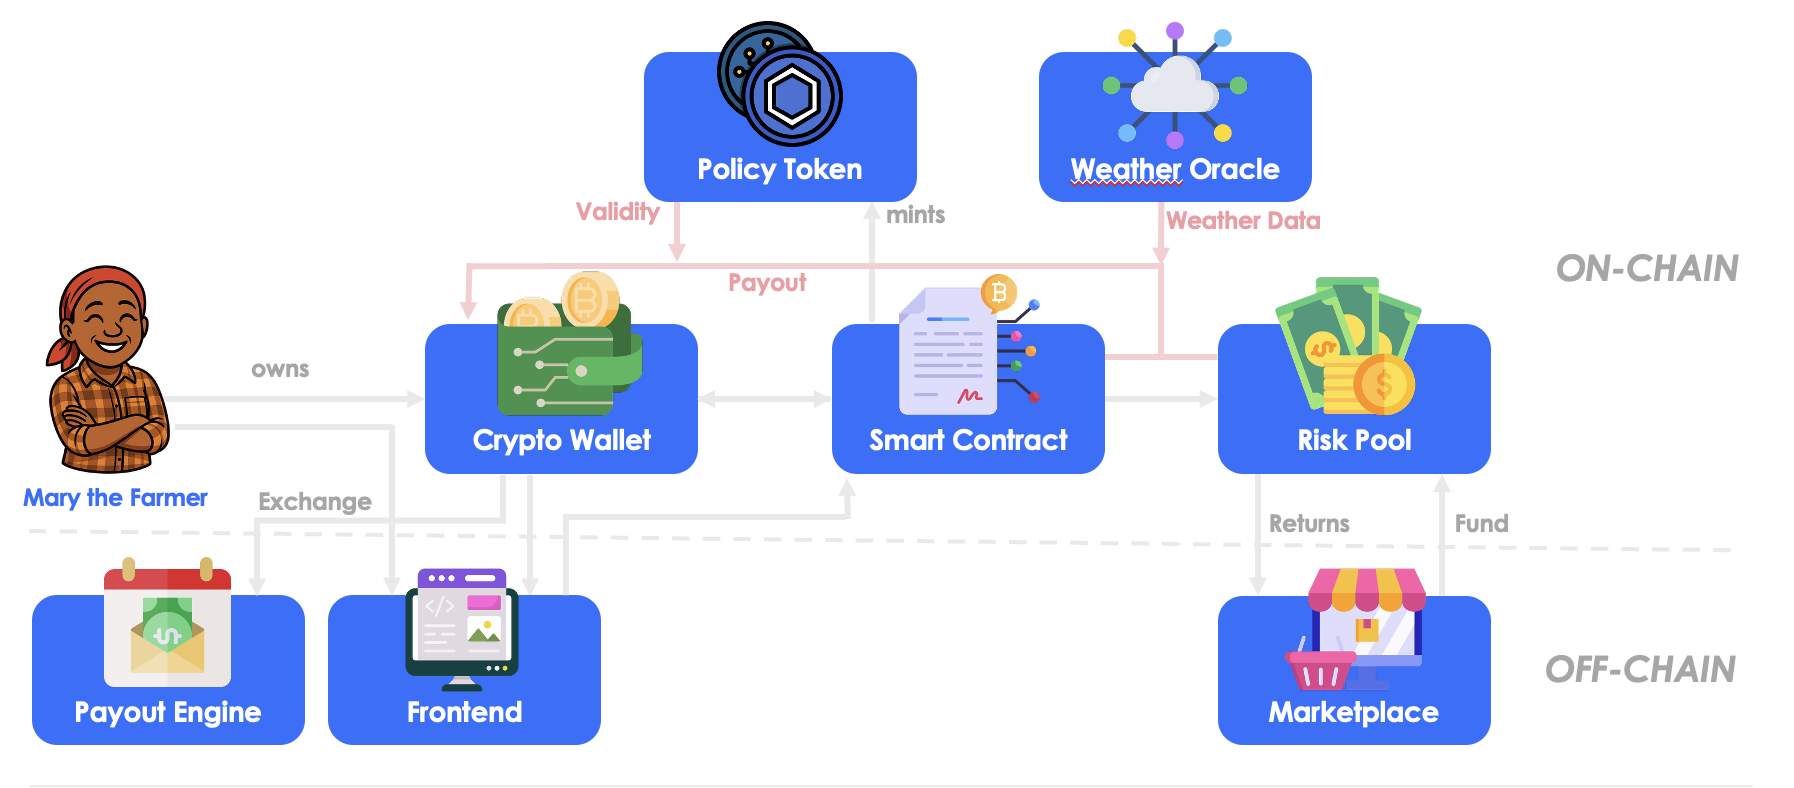
\includegraphics[scale=0.3]{graphics/Architectural_Overview}
		\caption{Architectural Overview \\ \textit{Source: Author's own.}}
		\label{fig:architecture}
	\end{figure}

	As shown in figure~\ref{fig:architecture} the users (both farmers and investors) own a crypto wallet and connect this to the frontend.
	The frontend then allows them to easily invest or buy policies for the current season with their crypto funds, by programmatically interacting with the Smart Contract.
	The smart contract then mints a policy token for farmers or deposits the investors funds in the vault, so that they can receive a yield.
	All funds are stored in a Risk-Pool (in our case the ERC4626 vault).
	The farmers can claim their policies at the end of the season and, if all conditions are met, i.e.\ the weather oracle gets and returns weather data, below the threshold and the farmer making the claim actually owns the policy tokens, receive their coverage funds.
	Investors may withdraw their funds, receiving all the accumulated yield.
	The \texttt{Payout Engine} symbolizes the possibility of transferring out funds from the crypto wallet to widely used mobile-money services, like M-Pesa.
	This is already a well established process and not included in the project itself, should however be noted, because it allows the farmers to actually immediately use their payouts in their everyday life.

	The concrete timeline for the process is based on the crop season and has 5 phases:
	\begin{enumerate}
		\item \textbf{Active Phase:} In the active phase policies can be bought and investments can be made.
			The premium for the current season is already set at the beginning through the auction-based system explained in section~\ref{sec:business-model} \textcolor{red}{check wether this links correctly!}.
			No claims or withdrawals can be made during this phase.
		\item \textbf{Inactive Phase:} Now the policies can no longer be bought, but investments can still be made.
			This allows for a speculative market for the insurance policies, while keeping the possibility of introducing more liquidity from capital investors.
		\item \textbf{Claim Phase:} The claim phase starts upon the actual crop season ending.
			Farmers may now try to claim their policies and receive their coverage payouts, while investors have to wait until this phase is over.
		\item \textbf{Withdrawal Phase:} Now investors may choose to withdraw their capital and receive their yield, while farmers wait until the next season is started.
		\item \textbf{Finished Phase:} The season is over, unclaimed policies are now invalid and not-withdrawn investments are used as liquidity for the next season, earning yield on the current investment (including the earned yield), creating a compounding effect.
        \label{enum:phases}
	\end{enumerate}

	% 3.3 Smart Contract Design (Micro)
	\subsection{Smart Contract Design (Micro)}\label{subsec:smart-contract-design}
	The project is built around a Solidity smart contract using the Ethereum Virtual Machine.
	This central RainyDayFund contract can be called using the front end and holds all the exposed functionality for the consumer.
	Investors use the \texttt{invest()} and \texttt{withdraw()} methods while insurees can buy and claim their policies in batches using the \texttt{buyPolicy()} and \texttt{claimPolicies()} functions.
	The contract leverages the ERC1155 token standard for policy tokens, enabling efficient batch operations and flexible policy management.

	As shown in Figure~\ref{fig:initial-contract-design}, the initial contract made use of the \texttt{1155 token standard} for the \texttt{policyTokens}, to take advantage of the cost-efficient batch operations~\parencite{ERC1155}.
	To help with testing the (Mock)-MUSCD was created, implementing the ERC20 interface, to emulate the behavior of common stablecoins like USDC, which are used as payment and funding for the riskpool.
	This allowed for the free minting and full control over the coins and made testing the functionality of the main contract possible, even within the bounds of Remix VM .
	Therefore, testing was quicker and easier at the beginning, without the need to always deploy on the Sepolia Testnet or an immediate, complete setup, for example with hardhat.

	Initially there were multiple issues:
	\begin{enumerate}[1]
		\item \textbf{Mapping for storing addresses:} Initially we used a mapping to store who had bought policies and was thereby eligible to claim them.
			However, there were some issues with this: Firstly, the policies lost all their value when they were resold, because the address of the new owner would not be tracked in the mapping.
			Moreover, storing all of this data was very gas-inefficient and redundant, because ownership of the policyToken is proof of ownership for the policy.
		\item \textbf{No proper incentive for investors:} We had already planned to give the investors some incentive to keep their funds in the riskpool, even after the season would end, to increase liquidity for the next season.
			The idea to achieve this, was, to use compound interest or create some other form of yield over time.
			However, implementing this with the initial setup proved difficult and created vastly unfair results \textcolor{red}{Hier vllt nochmal genauer erkl\"aren}
		\item \textbf{Weather oracle:} The initial mock-up for the weather oracle was just a number that could be accessed and stored on the contract directly.
			This was far from the goal of using chainlink as a decentralized oracle to reliably and transparently access the data.
		\item \textbf{Attack vectors:} Lastly there were some attack-vectors, especially for the owner.
			The \texttt{startNewSeason()} function could be used at any point during the season, thus rendering unclaimed policyTokens worthless and not allowing for investment-withdrawals to be made.
	\end{enumerate}

	\begin{figure}[H]
		\centering
		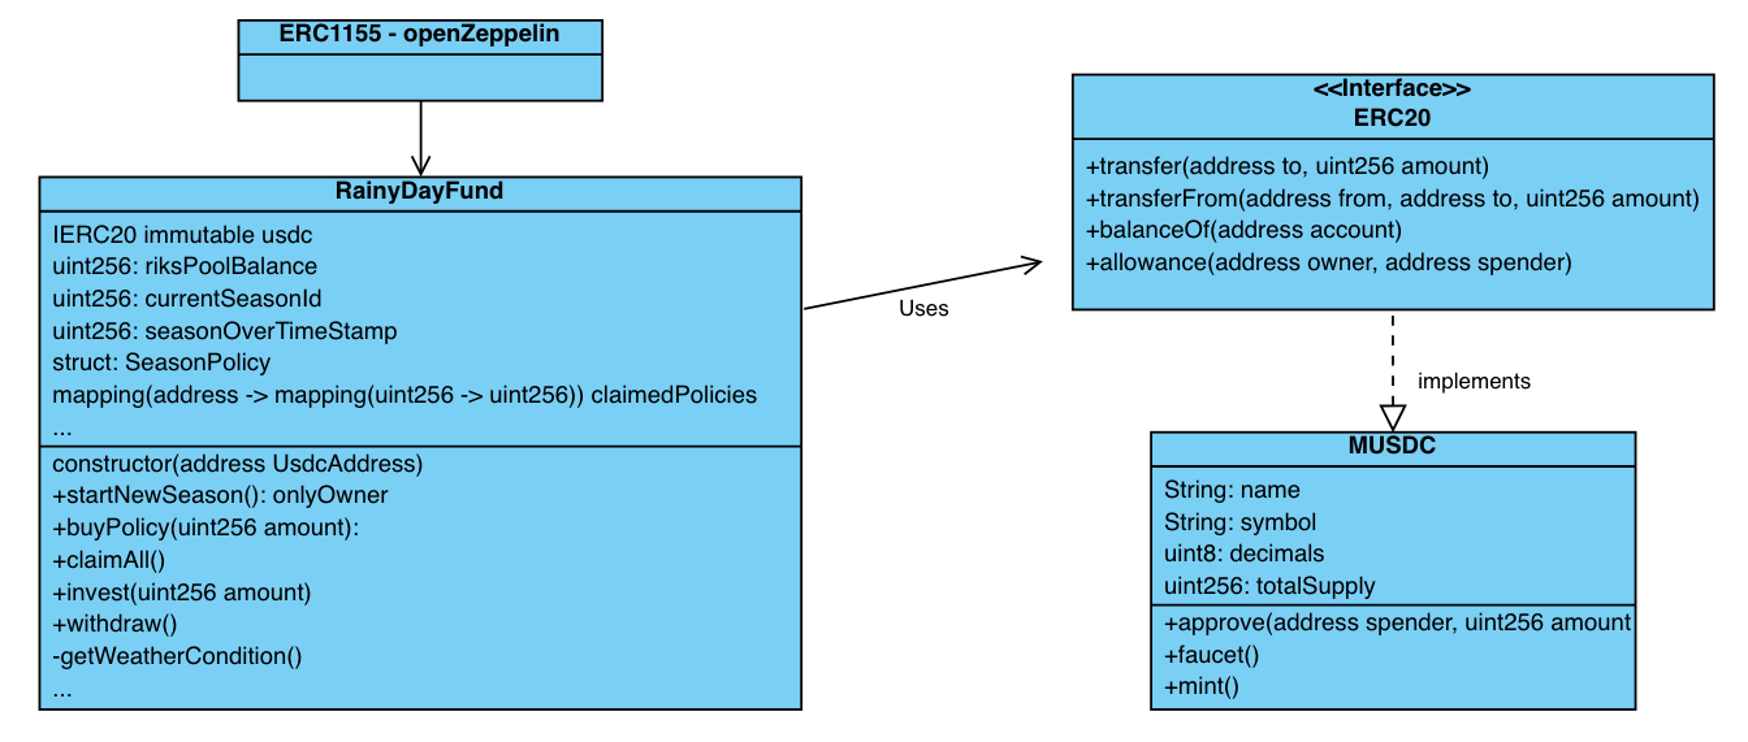
\includegraphics[scale=0.5]{graphics/ClassDiagram_Old}
		\caption{Initial Contract Design \\ \textit{Source: Author's own.}}
		\label{fig:initial-contract-design}
	\end{figure}

	Addressing these issues of the initial prototype the contract was restructured.
    The main fixes were:

    % Table: Major Issues and Fixes
    \begin{table}[H]
        \centering
        \caption{Major Issues and Corresponding Fixes}
        \label{tab:issues-fixes}
        \begin{tabular}{|p{0.42\textwidth}|p{0.42\textwidth}|}
            \hline
            \textbf{Issue} & \textbf{Fix} \\
            \hline
            Mapping for storing addresses was gas-inefficient and did not track policy resales & Removed the mapping \\
            \hline
            No proper incentive for investors and difficulties with implementation & Switched from self-made investment tracking to using the \texttt{ERC4626 vault} \\
            \hline
            Using Token Standards ERC4626, ERC20 and ERC1155 simultaneously, causing errors with inheritance of the contract & Switched from ERC1155 to only using ERC20 for the policyTokens \\
            \hline
            Weather Oracle / Chainlink integration & Implementing the proper Chainlink standards for the mock-up-weather oracle~\parencite{AggregatorV3Interface} \\
            \hline
            Attack Vector for Owner & Fixed some issues by including modifiers and properly implementing \enquote{mini-}state-machine (refer to enumeration~\ref{enum:phases}) \\
            \hline
        \end{tabular}
    \end{table}

    The final state of the contract can be seen here:

    \begin{figure}[H]
        \centering
        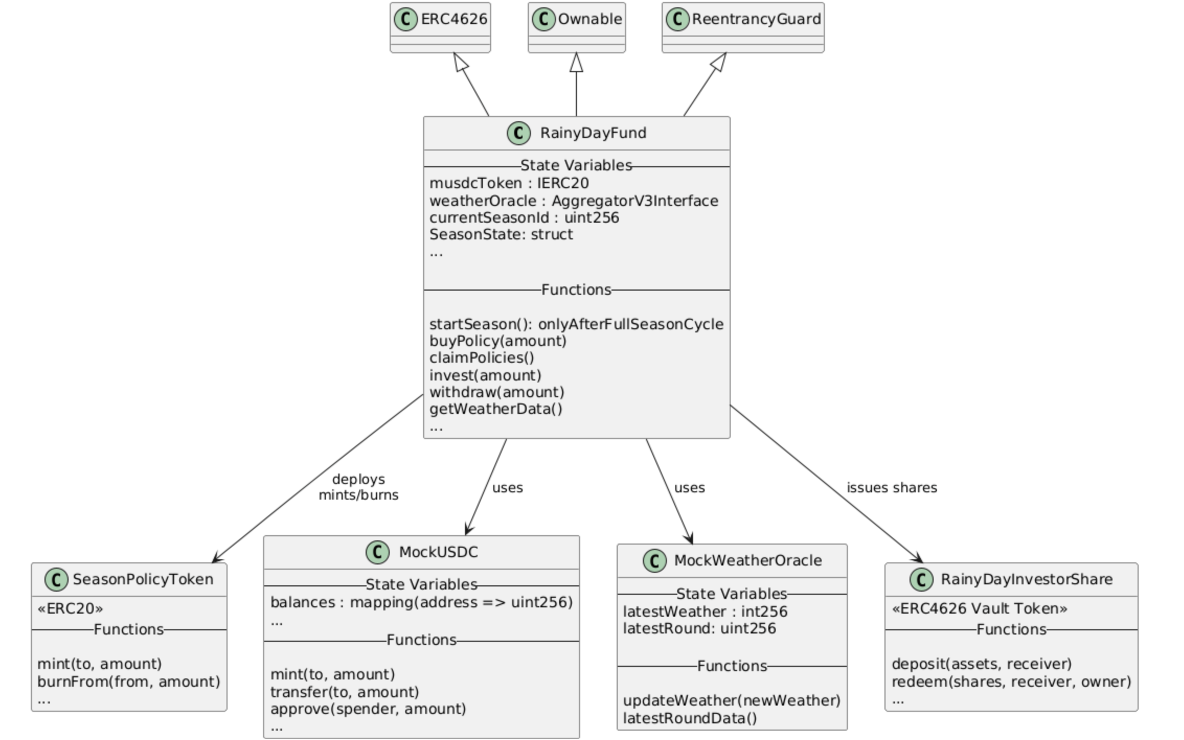
\includegraphics[scale=0.5]{graphics/ClassDiagram_New}
        \caption{Final Contract Design \\ \textit{Source: Author's own.}}
        \label{fig:final-contract-design}
    \end{figure}


	% 3.4 Developmnet Tools & Infrastructure 
	\subsection{Development Tools \& Infrastructure}\label{subsec:development-tools-infrastructure}
	The development process utilized a modern toolchain centered around the Hardhat framework for smart contract development, deployment and testing.
	For the smart contract development, we first used the Remix IDE, which allowed for easy deployment and manual testing directly in the browser without any setup requirements.
	Once we had a working prototype, we transitioned to Hardhat, which provided a more robust development environment with a local blockchain that simulates real network conditions.
	The frontend was built using React, providing an interface to manually test our contracts and demonstrate functionality.
	Throughout our project, we used version control via git and explicitly a GitHub repository, which made collaboration between team members flawless and provided accountability measures in case of errors.
	For deployment, we initially planned on using the Sepolia testnet, but in the final sprint decided to only deploy it locally.
	The reason for this is a multitude of problems arising when we tried it via Sepolia - while we managed to get as far as deploying, interacting with the contracts turned out too difficult within this timeframe.
	The compromise was made: use local network only, but in return we managed to get a fully working prototype that runs predictably without external dependencies.
	For development environments, we used the Remix IDE initially for its straightforward Solidity development capabilities, and later Neovim for anything that wasn't written in Solidity.
	All deployment was handled through JavaScript files within the Hardhat framework. 

	% 3.5 Quality Assurance & Security
	\subsection{Quality Assurance \& Security}\label{subsec:qa-security}
	Our quality assurance strategy focused on comprehensive testing and systematic validation of contract functionality.
	All tests were written in TypeScript using the Node.js framework with Chai for assertions, which helped catch errors early and made the code easier to maintain.
	To ensure thorough testing without external dependencies, we created MockUSCD, an ERC20 token that behaves like USDC, allowing us to test all payment and funding functionality for the risk pool without needing real money or external services.
	This approach enabled complete control over the testing environment and made testing the functionality of the main contract possible even within controlled VM environments.
	The test setup, as shown in Figure~\ref{fig:test-set-up}, highlights the importance of robust testing and code coverage in the project.
	Our test coverage reaches nearly 100\% on critical functions, which helped catch bugs early when they were still easy to fix.
	The comprehensive test suite verifies the contract works correctly across different scenarios, including edge cases and potential attack vectors.

	\begin{figure}[H]
		\centering
		\begin{minipage}[b]{0.48\textwidth}
			\centering
			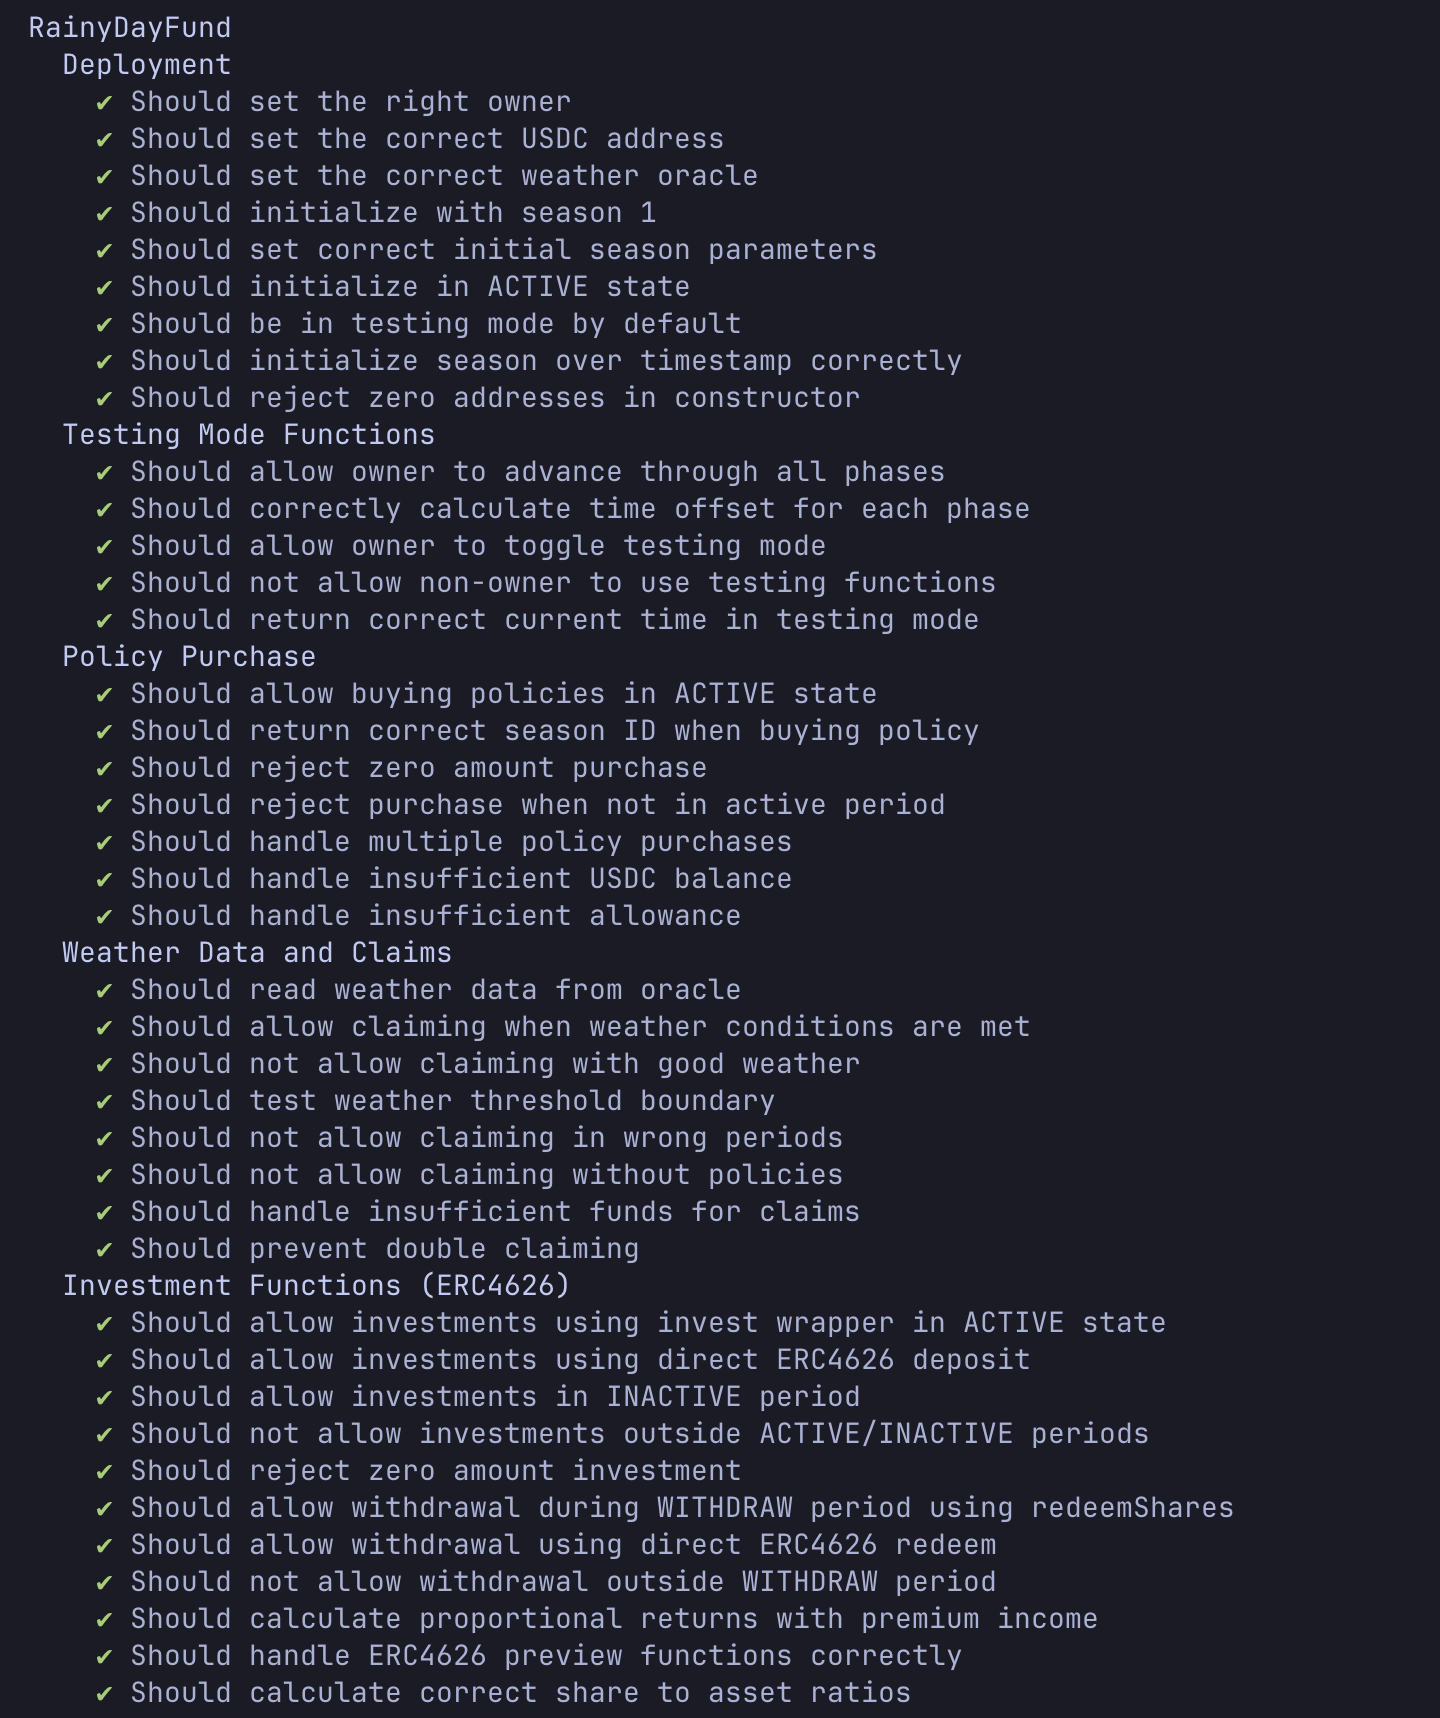
\includegraphics[width=0.95\linewidth]{graphics/Passing_Tests}
			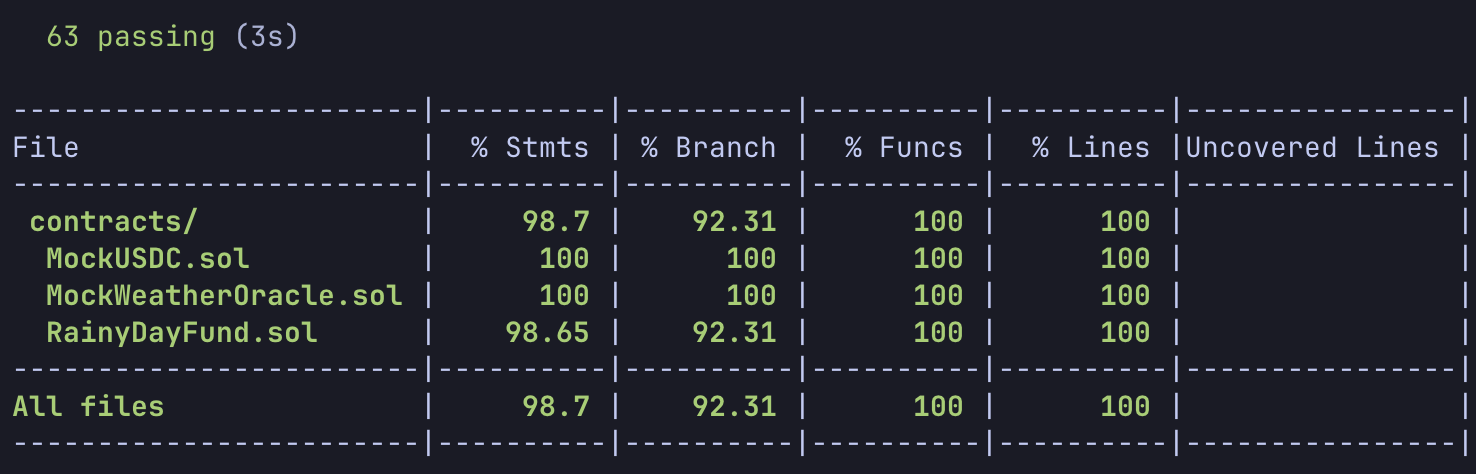
\includegraphics[width=0.95\linewidth]{graphics/Test_Coverage}
			\caption*{(a) Passing Tests and Coverage}
		\end{minipage}\hfill
		\begin{minipage}[b]{0.48\textwidth}
			\centering
			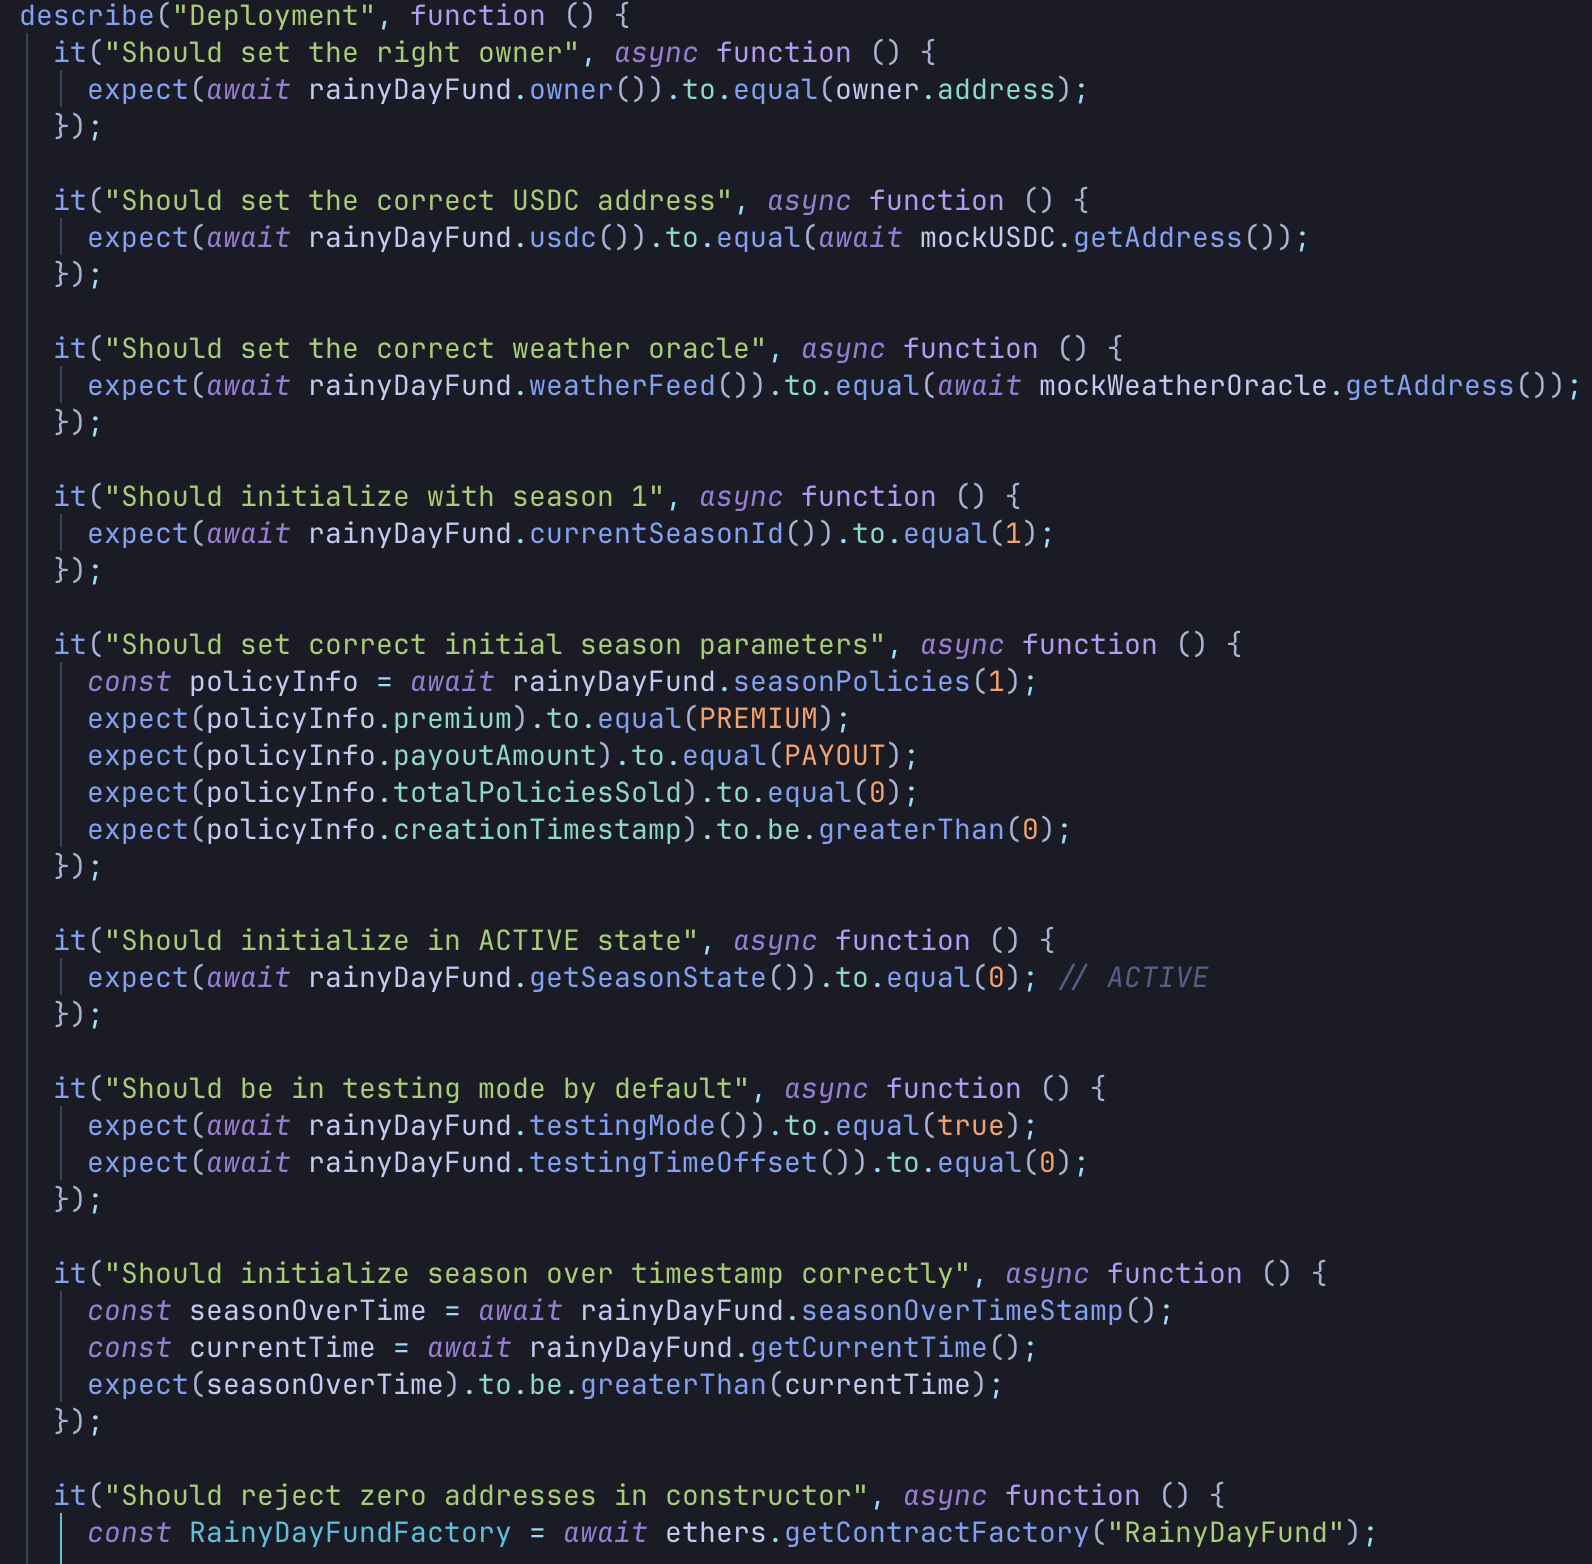
\includegraphics[width=0.95\linewidth]{graphics/Test_Code}
			\caption*{(b) Test Code}
		\end{minipage}
		\caption{Test Setup. (a) Passing tests and coverage; (b) Excerpt of test code. \\ \textit{Source: Author's own.}}
		\label{fig:test-set-up}
	\end{figure}

	% 3.6 Outlook & Next Steps
	\subsection{Outlook \& Next Steps}\label{subsec:outlook}
	The most important next step is integrating real Chainlink oracles for weather data.
	Right now we're using mock data, but production needs reliable, tamper-proof weather information from multiple sources.
	We'll also need to deploy on a real network.
	Layer 2 solutions like Polygon or Arbitrum make sense because gas costs are much lower - important when your users are price-sensitive farmers.
	We might also look into cross-chain deployment to give users more options.
	The smart contract architecture needs some work for production.
	We'll want upgradeability mechanisms so we can fix bugs and add features, but we need to balance that with immutability for user trust.
	Gas optimization is another priority - the current contract works but isn't optimized for cost.
	For additional features, we're thinking about crop-specific insurance products and multi-season coverage.
	The current single-season model is too limiting for real-world agriculture.
	We'd also like to support group policies for farmer cooperatives.
	The frontend needs to be much more user-friendly, especially for people with limited digital experience.
	Mobile-first design is essential since most users will access this through smartphones.
	We'll need offline capabilities too since internet connectivity can be spotty in rural areas.
	Technical priorities include:

	\begin{enumerate}
		\item Chainlink integration for real weather data
		\item Layer 2 deployment for lower costs
		\item Gas optimization and contract upgrades
		\item Mobile-optimized frontend with offline support
		\item Multi-language support and simplified interfaces
	\end{enumerate}

	We're also planning more comprehensive testing on testnets once we sort out the deployment issues.
	The current local testing is good for development, but we need real network conditions to catch problems we haven't thought of.


	% 4 Conclusion
	\section{Conclusion}\label{sec:conclusion}
	\ldots

	% ---------- Bibliography ----------
	\printbibliography

	\appendix
	\section*{Appendices}\label{sec:appendix}
	Add any supplementary material here.

\end{document}
